\subsection{Description of the CNRS Benchmark} \label{sec:benchmark}

The CNRS Benchmark \cite{tiberga_results_2020} is a numerical
benchmark for multiphysics software dedicated to modeling \glspl{MSR}. It
consists of three phases and eight steps in total. Each
step is a well-defined subproblem for systematically assessing the
capabilities of \gls{MSR} software and pinpointing sources of discrepancies
between software. Phase 0 consists of three single-physics problems in fluid
dynamics, neutronics, and temperature. Phase 1 consists
of four coupled steady-state problems. Lastly, Phase 2 consists of one
coupled, time-dependent problem.

\begin{figure}[htb!]
	\centering
	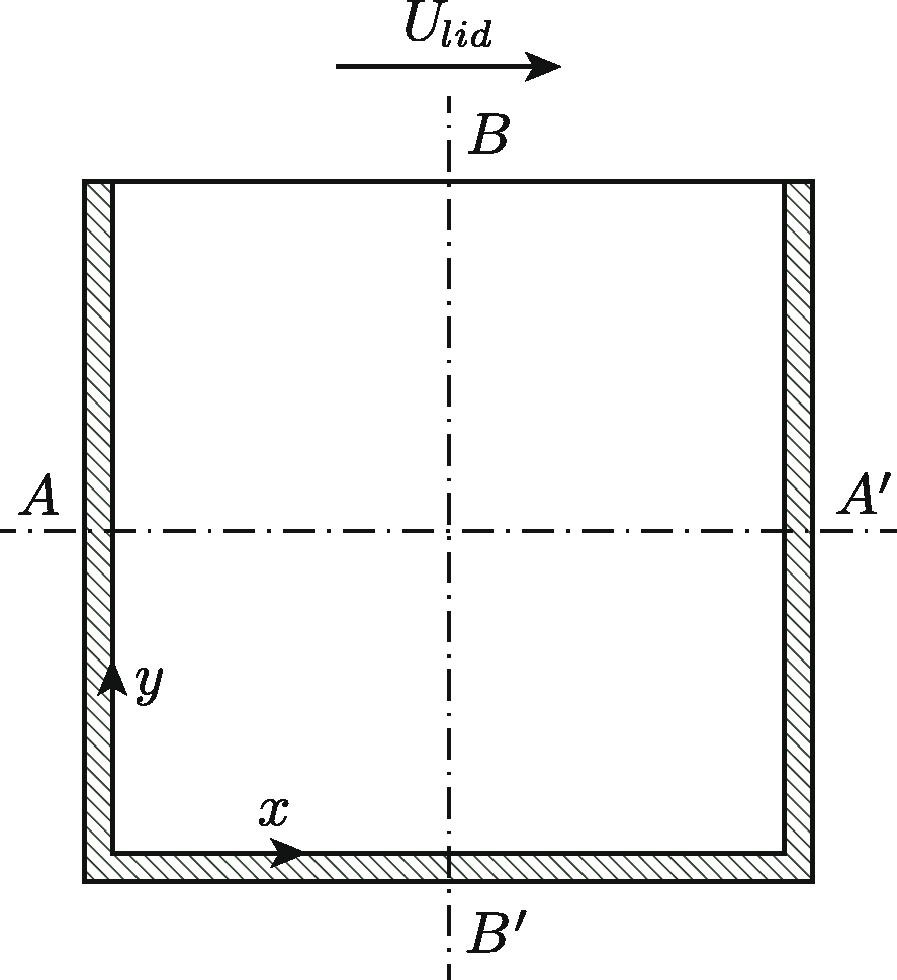
\includegraphics[width=.6\columnwidth]{cnrs-geometry}
	\caption{2m$\times$2m 2D domain of the CNRS Benchmark. $U_{lid}$
	represents the velocity along the top boundary. For comparison, various quantities are
	measured along the centerlines AA' and BB'. From Tiberga et
	al. \cite{tiberga_results_2020}.}
	\label{fig:cnrs-geometry}
\end{figure}

As shown in Figure \ref{fig:cnrs-geometry}, the domain geometry is a
2m$\times$2m square cavity filled with LiF-BeF$_2$-UF$_4$ molten salt at an
initial temperature of 900K \cite{tiberga_results_2020}.
Standard vacuum boundary conditions apply for neutron flux along all
boundaries whereby outgoing neutrons are considered lost, while homogeneous
boundary conditions apply for delayed neutron precursors. No-slip boundary
conditions apply for velocity variables in the cavity, except along the top
boundary for Steps 0.1, 0.3, 1.1, 1.2, and 1.4, which impose forced flow in the
form of lid-driven
cavity flow. For the temperature variable, all boundaries are insulated, and we
simulate salt cooling with the following volumetric heat sink equation:
%
\begin{align}
    q'''(\vec{r}) &= \gamma \left(900 - T(\vec{r})\right) \label{eq:cnrs-heat}
    \shortintertext{where}
    q''' &= \mbox{volumetric heat sink [W$\cdot$m$^{-3}$],}
    \nonumber \\
    \gamma &= \mbox{heat transfer coefficient [W$\cdot$m$^{-3}\cdot$K$^{-1}$],}
    \nonumber \\
    T(\vec{r}) &= \mbox{temperature at point $\vec{r}$ [K].} \nonumber
\end{align}

Tiberga et al. \cite{tiberga_results_2020} used Serpent 2
\cite{leppanen_serpent_2014} with the JEFF-3.1 library
\cite{koning_jeff-31_2006} to generate multigroup neutronics data for the
LiF-BeF$_2$-UF$_4$ salt in the domain at 900K, which they condensed into six
energy groups and eight precursor groups. We direct readers to their paper for
the group constant data \cite{tiberga_results_2020}. In addition, the
benchmark prescribes the following equations to govern the temperature
dependence in the cross sections and the neutron diffusion coefficients:
%
\begin{align}
    \Sigma_i (T) &= \Sigma_i(T_{ref})
    \frac{\rho_{fuel}(T)}{\rho_{fuel}(T_{ref})}
    \shortintertext{and}
    D (T) &= D(T_{ref})
    \frac{\rho_{fuel}(T_{ref})}{\rho_{fuel}(T)}
    \shortintertext{where}
    \Sigma_i &= \mbox{relevant macroscopic cross section [cm${-1}$],}
    \nonumber \\
    D &= \mbox{neutron diffusion coefficient [cm$^2\cdot$s$^{-1}$],}   
    \nonumber \\
    \rho_{fuel} &= \mbox{density of the fuel salt [kg$\cdot$m$^{-3}$],}
    \nonumber \\
    T_{ref} &= \mbox{reference temperature} = 900\mbox{ K}. \nonumber
\end{align}

The benchmark also prescribes incompressible Navier-Stokes flow with the
Boussinesq approximation for evaluating the salt flow in the
domain but does not restrict the type of neutronics model.
Table \ref{table:benchmark} lists the relevant input parameters and observables.

\begin{table*}[tp!]
	\caption{Input parameters and observables of each benchmark step.}
	\centering
	\footnotesize
    \begin{tabular}{p{.05\textwidth} p{.1\textwidth} p{.3\textwidth} p{.45\textwidth}}
		\toprule
        \textbf{Step} & \textbf{Name} & \textbf{Input parameters} & \textbf{Observables} \\
		\midrule
        0.1 & Velocity field &
		\begin{itemize}[nosep,noitemsep,left=0pt,
		                before={\begin{minipage}[t]{\hsize}},
                        after ={\end{minipage}}]
		    \item $U_{lid} = 0.5$ m$\cdot$s$^{-1}$
		\end{itemize}\vspace*{-\baselineskip}\mbox{} &
		\begin{itemize}[nosep,noitemsep,left=0pt,
		                before={\begin{minipage}[t]{\hsize}},
                        after ={\end{minipage}}]
		    \item Velocity components $(u_x,u_y)$ along AA' and BB'
		\end{itemize}\vspace*{-\baselineskip}\mbox{} \\
        \midrule
        0.2 & Neutronics &
        \begin{itemize}[nosep,noitemsep,left=0pt,
		                before={\begin{minipage}[t]{\hsize}},
                        after ={\end{minipage}}]
		    \item $U_{lid} = 0$ m$\cdot$s$^{-1}$
		    \item $T = 900$ K
		    \item $P = 1$ GW
		\end{itemize} &
		\begin{itemize}[nosep,noitemsep,left=0pt,
		                before={\begin{minipage}[t]{\hsize}},
                        after ={\end{minipage}}]
		    \item Fission rate density $\sum^6_g \Sigma_{f,g} \phi_g(\vec{r})$ along AA'
            \item Reactivity $\rho$
		\end{itemize}\vspace*{-\baselineskip}\mbox{} \\
        \midrule
        0.3 & Temperature &
        \begin{itemize}[nosep,noitemsep,left=0pt,
		                before={\begin{minipage}[t]{\hsize}},
                        after ={\end{minipage}}]
		    \item Fixed flow field from Step 0.1 for
		    $U_{lid} = 0.5$ m$\cdot$s$^{-1}$
		    \item Fixed heat source distribution
		    $\sum^6_{g} \epsilon_g \Sigma_{f,g} \phi_g(\vec{r})$ from Step 0.2
		    \item $\gamma = 10^6$ W$\cdot$m$^{-3}\cdot$K$^{-1}$
		\end{itemize} &
		\begin{itemize}[nosep,noitemsep,left=0pt,
		                before={\begin{minipage}[t]{\hsize}},
                        after ={\end{minipage}}]
		    \item Temperature $T$ along AA' and BB'
		\end{itemize}\vspace*{-\baselineskip}\mbox{} \\
        \midrule
        1.1 & Circulating fuel &
        \begin{itemize}[nosep,noitemsep,left=0pt,
		                before={\begin{minipage}[t]{\hsize}},
                        after ={\end{minipage}}]
		    \item Fixed flow field from Step 0.1 for
		    $U_{lid} = 0.5$ m$\cdot$s$^{-1}$
		    \item $T = 900$ K
		    \item $P = 1$ GW
		\end{itemize} &
		\begin{itemize}[nosep,noitemsep,left=0pt,
		                before={\begin{minipage}[t]{\hsize}},
                        after ={\end{minipage}}]
		    \item Delayed neutron source $\sum^8_i \lambda_i C_i$ along AA' and BB'
		    \item Reactivity change between Step 1.1 and Step 0.2,
		    $\Delta \rho = \rho - \rho_{s_{0.2}}$
		\end{itemize}\vspace*{-\baselineskip}\mbox{} \\
        \midrule
        1.2 & Power coupling &
        \begin{itemize}[nosep,noitemsep,left=0pt,
		                before={\begin{minipage}[t]{\hsize}},
                        after ={\end{minipage}}]
		    \item Fixed flow field from Step 0.1 for
		    $U_{lid} = 0.5$ m$\cdot$s$^{-1}$
		    \item $P = 1$ GW
		    \item $\gamma = 10^6$ W$\cdot$m$^{-3}\cdot$K$^{-1}$
		\end{itemize}\vspace*{-\baselineskip}\mbox{} &
		\begin{itemize}[nosep,noitemsep,left=0pt,
		                before={\begin{minipage}[t]{\hsize}},
                        after ={\end{minipage}}]
		    \item Temperature $T$ along AA' and BB'
            \item Reactivity change between Step 1.2 and Step 1.1,
            $\Delta\rho = \rho - \rho_{s_{1.1}}$
            \item Change in fission rate density
            $\sum^6_g \Sigma_{f,g} \phi_g(\vec{r}) -
            \left[\sum^6_g \Sigma_{f,g} \phi_g(\vec{r})\right]_{s_{0.2}}$
		\end{itemize} \\
        \midrule
        1.3 & Buoyancy &
        \begin{itemize}[nosep,noitemsep,left=0pt,
		                before={\begin{minipage}[t]{\hsize}},
                        after ={\end{minipage}}]
		    \item $P = 1$ GW
		    \item $U_{lid} = 0$ m$\cdot$s$^{-1}$
		    \item $\gamma = 10^6$ W$\cdot$m$^{-3}\cdot$K$^{-1}$
		\end{itemize}\vspace*{-\baselineskip}\mbox{} &
		\begin{itemize}[nosep,noitemsep,left=0pt,
		                before={\begin{minipage}[t]{\hsize}},
                        after ={\end{minipage}}]
		    \item Velocity components $(u_x, u_y)$ along AA' and BB'
            \item Temperature $T$ along AA' and BB'
            \item Delayed neutron source $\sum^8_i \lambda_i C_i$ along AA' and BB'
            \item Reactivity change from Step 0.2
        $\Delta\rho = \rho - \rho_{s_{0.2}}$
		\end{itemize} \\
        \midrule
        1.4 & Full coupling &
        \begin{itemize}[nosep,noitemsep,left=0pt,
		                before={\begin{minipage}[t]{\hsize}},
                        after ={\end{minipage}}]
		    \item $\gamma = 10^6$ W$\cdot$m$^{-3}\cdot$K$^{-1}$
		    \item $P$ variable in the range $[0,1]$ GW with a step of 0.2 GW
		    \item $U_{lid}$ variable in the range $[0,0.5]$ m$\cdot$s$^{-1}$
		    with a step of 0.1 m$\cdot$s$^{-1}$
		\end{itemize} &
		\begin{itemize}[nosep,noitemsep,left=0pt,
		                before={\begin{minipage}[t]{\hsize}},
                        after ={\end{minipage}}]
		    \item Reactivity change between Step 1.4 and Step 0.2,
		    $\Delta\rho = \rho - \rho_{s_{0.2}}$, for all permutations of $P$
		    and $U_{lid}$ values
		\end{itemize}\vspace*{-\baselineskip}\mbox{} \\
        \midrule
        2.1 & Forced convection transient &
        \begin{itemize}[nosep,noitemsep,left=0pt,
		                before={\begin{minipage}[t]{\hsize}},
                        after ={\end{minipage}}]
		    \item $\gamma = 10^6$ W$\cdot$m$^{-3}\cdot$K$^{-1}$
            \item Steady-state solution from Step 1.4 for $U_{lid} = 0.5$
        m$\cdot$s$^{-1}$ and $P = 1.0$ GW
		\end{itemize} &
		\begin{itemize}[nosep,noitemsep,left=0pt,
		                before={\begin{minipage}[t]{\hsize}},
                        after ={\end{minipage}}]
		    \item Power gain and shift as a function of the perturbation frequency
		\end{itemize}\vspace*{-\baselineskip}\mbox{} \\
		\bottomrule
	\end{tabular}
	\label{table:benchmark}
\end{table*}

Step 2.1 studies the transient response of the fully coupled nonlinear system.
Linear perturbation analyses are performed by introducing periodic
perturbations to the heat transfer coefficient $\gamma$ and studying the gain
and phase shift of the response in the total power $P$. For the initial
conditions, the steady-state solution from Step 1.4 with
$U_{lid} = 0.5$ m$\cdot$s$^{-1}$ and $P = 1$ GW is used. This initial
configuration is made exactly critical by scaling the neutron source terms,
from fission and \gls{DNP} decay, by the inverse of the criticality eigenvalue
solution from Step 1.4.

$\gamma$ is uniformly perturbed according to small-amplitude sine waves given
as:
%
\begin{align}
    \gamma =& \gamma_0 \left[ 1 + 0.1\sin\left(2 \pi f \right) \right]
    \shortintertext{where}
    \gamma_0 =& 10^6 \mbox{ W$\cdot$m$^{-3}\cdot$K$^{-1}$}, \nonumber \\
    f \in& \left\lbrace 0.0125, 0.025, 0.05, 0.1, 0.2, 0.4, 0.8 \right\rbrace 
    \mbox{ Hz.} \nonumber
\end{align}

The benchmark defines power gain as:
%
\begin{align}
    \mbox{Power gain} =& \frac{\left(P_{max} - P_{avg}\right)/P_{avg}}{
    \left(\gamma_{max} - \gamma_{avg}\right)/\gamma_{avg}}
\end{align}
%
The subscripts denote the maximum and time-averaged values of $P$ and $\gamma$.

\FloatBarrier
